% Бүлэг 3

\chapter{Системийн зохиомж} % Зарим нэг зөвлөмж
\label{Chapter3} % Энэ бүлэг рүү ишлэл хийх бол \ref{Chapter2} командыг ашигла 
\newpage
\section{Өгөгдлийн ерөнхий схем:}
		\begin{figure}[h!]
			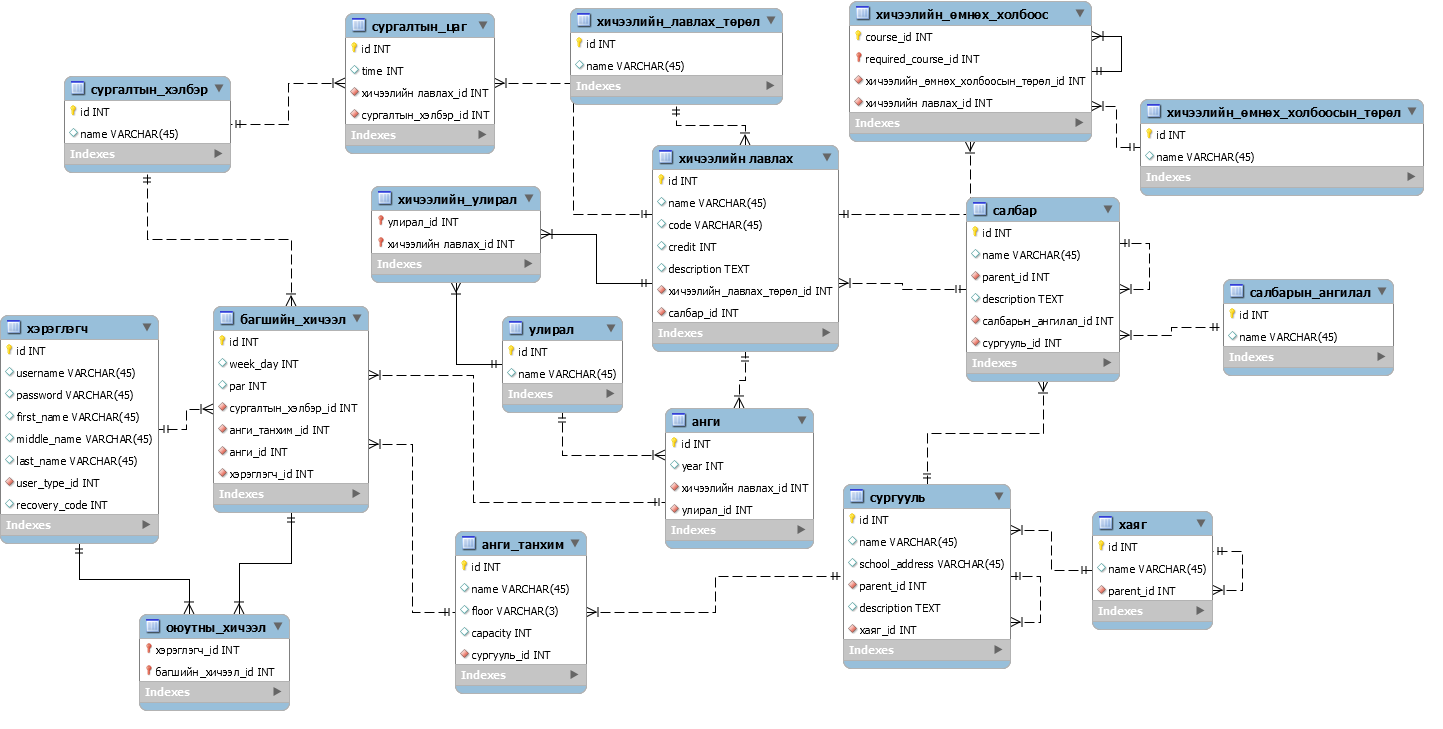
\includegraphics[angle=90, scale=0.4]{Diagrams/eschool_course}
			\caption[Өгөгдлийн ерөнхий схем]{Өгөгдлийн ерөнхий схем}
			\label{text}
		\end{figure}
\newpage	
\section{Класс диаграм}
	\begin{figure}[!h]
		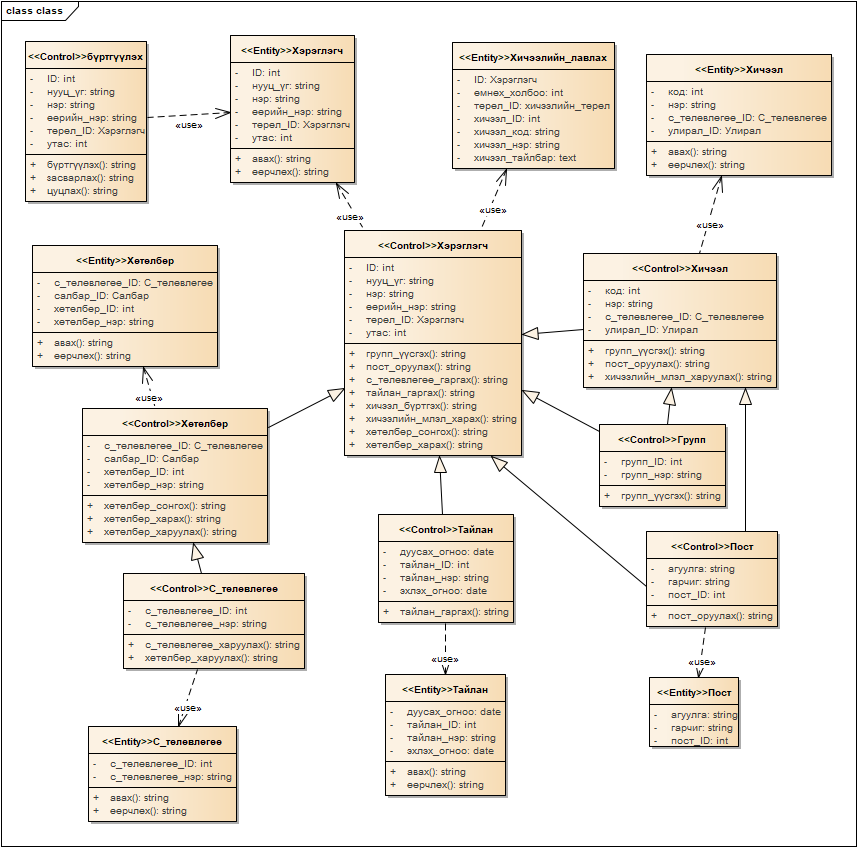
\includegraphics[angle=90,scale=0.5]{Diagrams/Class}
		\caption[Зохиомжийн шатны класс диаграм]{Зохиомжийн шатны класс диаграм}
		\label{text}
	\end{figure}
	
\newpage
\section{Хэрэглэгчийн интерфейс }

	\begin{figure}[!h]
		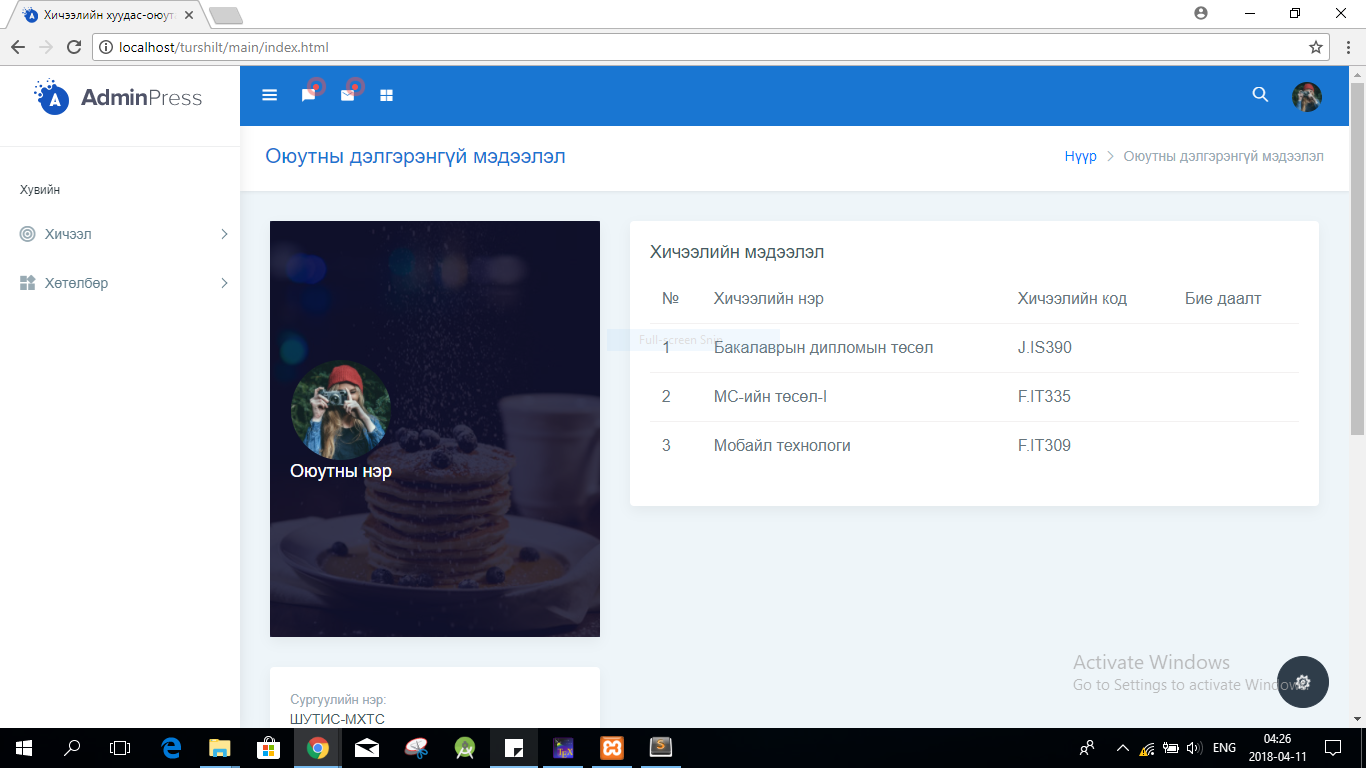
\includegraphics[scale=0.42]{Chart/screen-1}
		\caption[Оюутан харах нүүр хуудас]{Оюутан харах нүүр хуудас}
		\label{text}
	\end{figure}

	\begin{figure}[!h]
		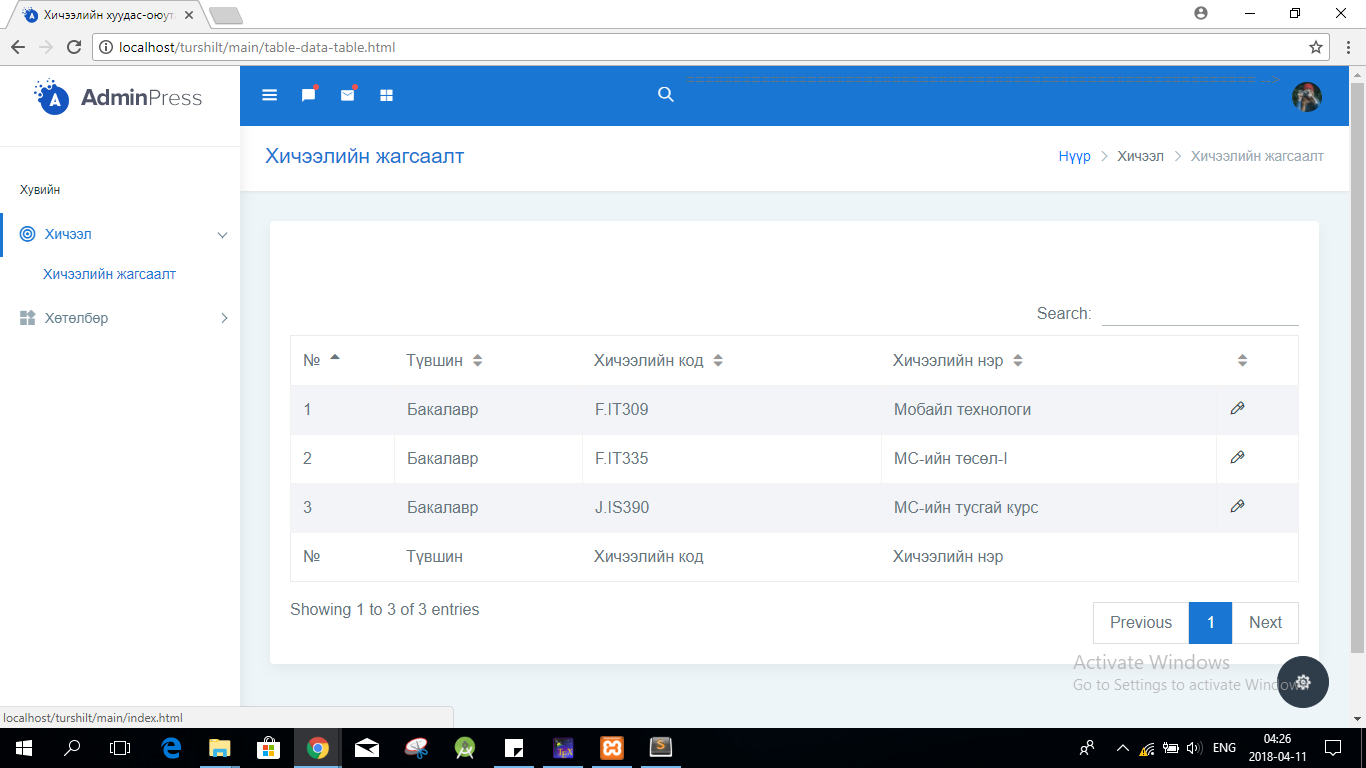
\includegraphics[scale=0.42]{Chart/screen-2}
		\caption[Оюутан хичээлийн жагсаалт харах]{Оюутан хичээлийн жагсаалт харах}
		\label{text}
	\end{figure}
	
	\begin{figure}[!h]
		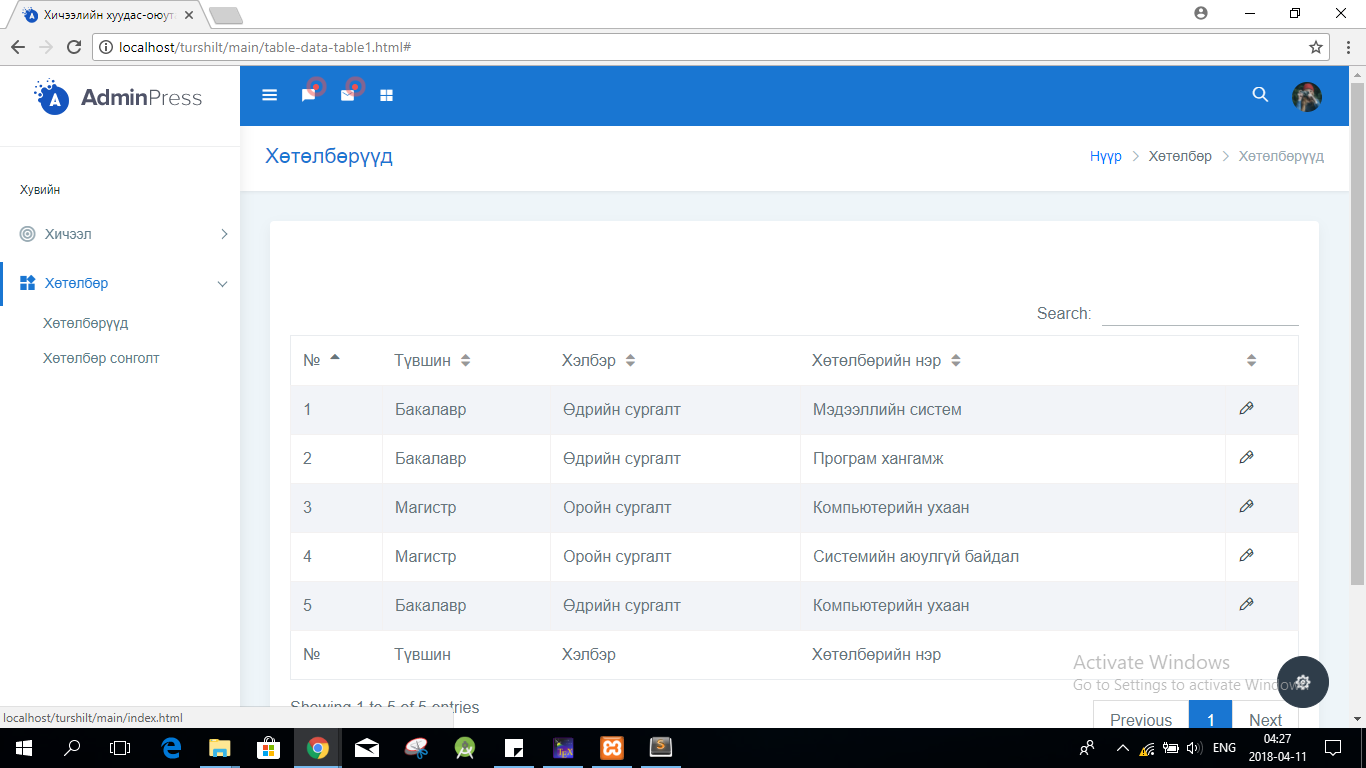
\includegraphics[scale=0.47]{Chart/screen-3}
		\caption[Оюутан хөтөлбөрийн мэдээлэл харах]{Оюутан хөтөлбөрийн мэдээлэл харах}
		\label{text}
	\end{figure}
	
	\begin{figure}[!h]
		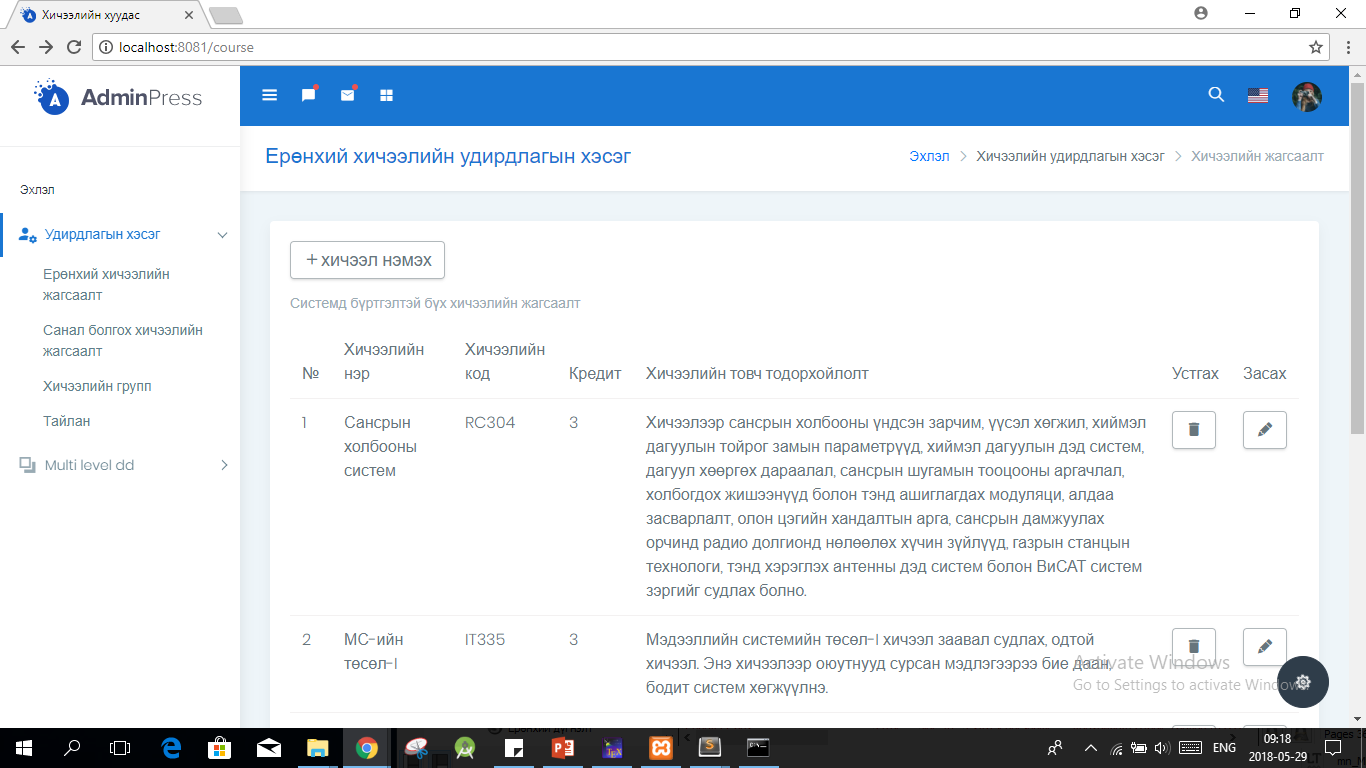
\includegraphics[scale=0.47]{Chart/screen-5}
		\caption[СА-ы ажилтан хичээл бүртгэх]{СА-ы ажилтан хичээл бүртгэх}
		\label{text}
	\end{figure}\begin{center}
	\begin{figure}[!h]
		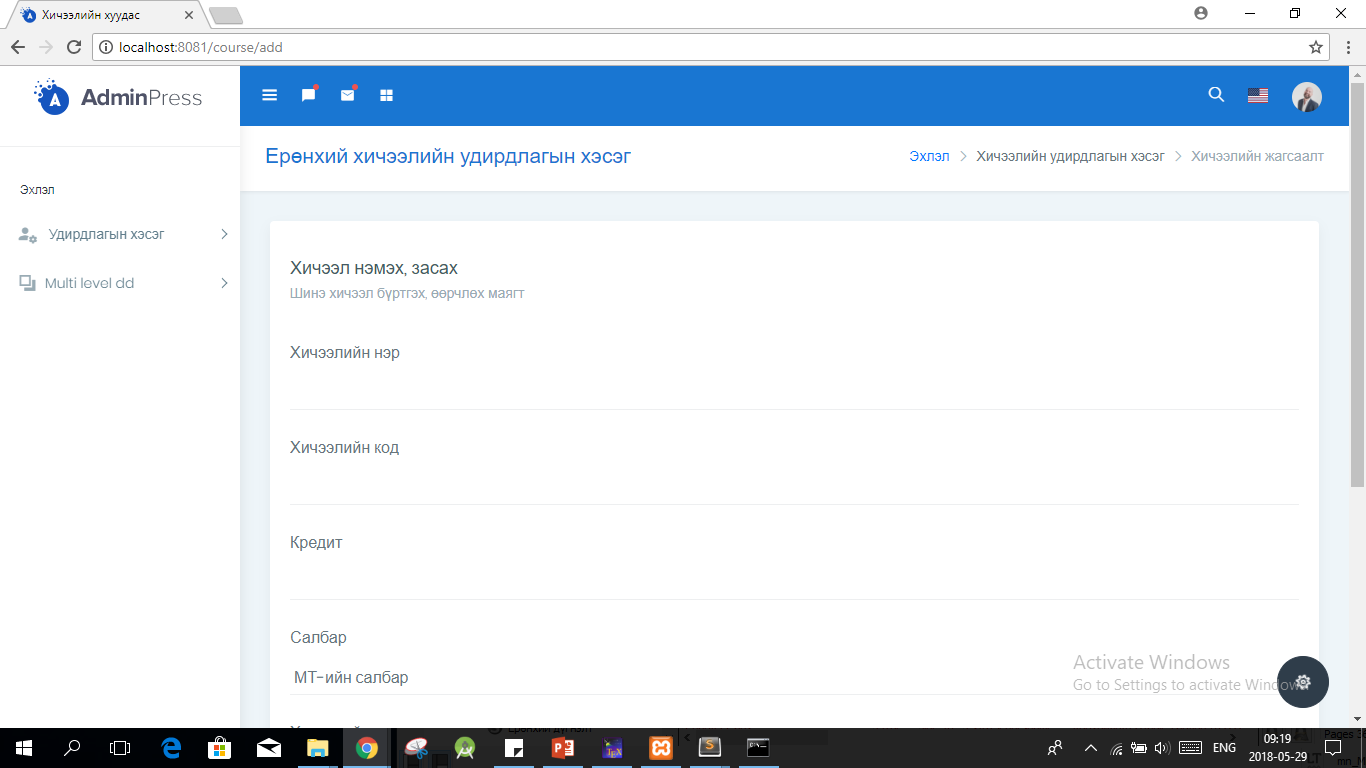
\includegraphics[scale=0.42]{Chart/screen-6}
		\caption[СА-ы ажилтан хичээл бүртгэх]{СА-ы ажилтан хичээл бүртгэх}
		\label{text}
	\end{figure}
\begin{figure}[!h]
	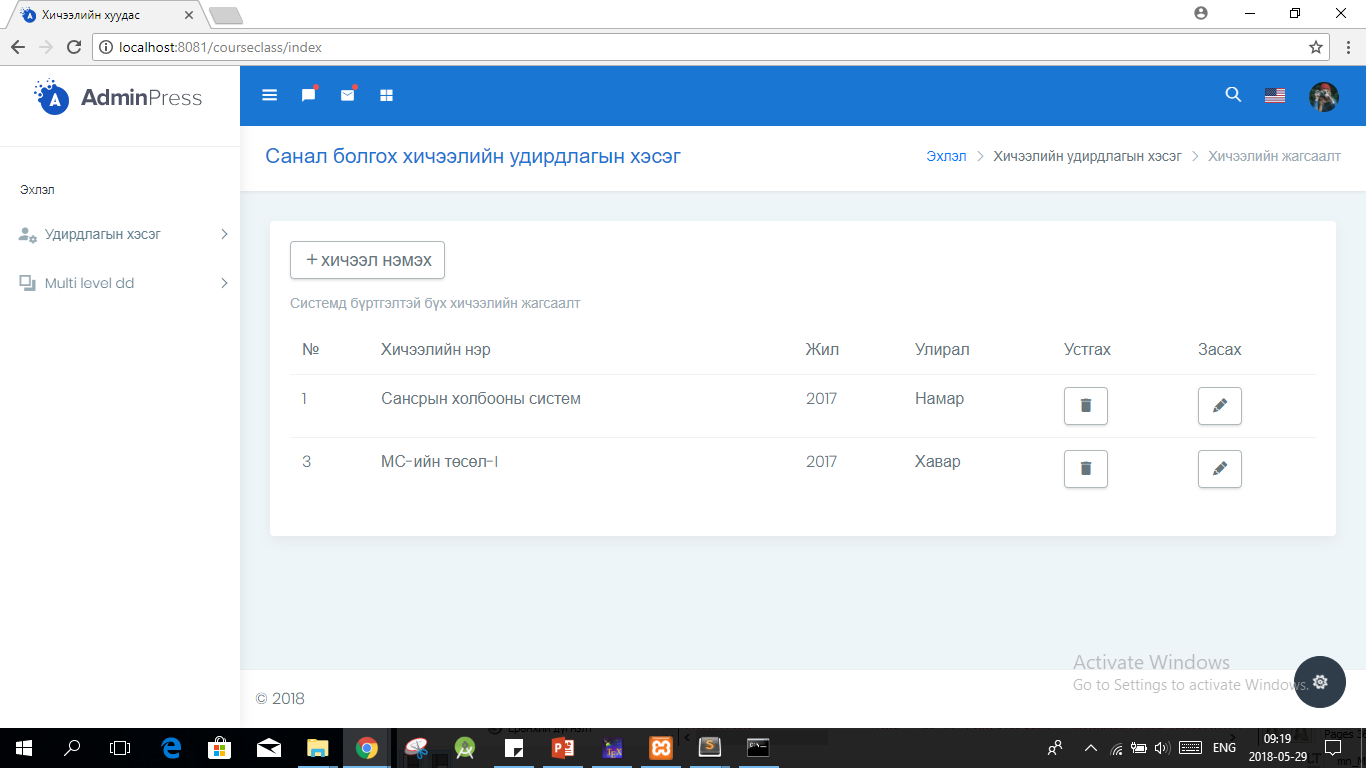
\includegraphics[scale=0.42]{Chart/screen-7}
	\caption[СА-ы ажилтан улирлын хичээл бүртгэх]{СА-ы ажилтан улирлын хичээл бүртгэх}
	\label{text}
\end{figure}
\begin{figure}[!h]
	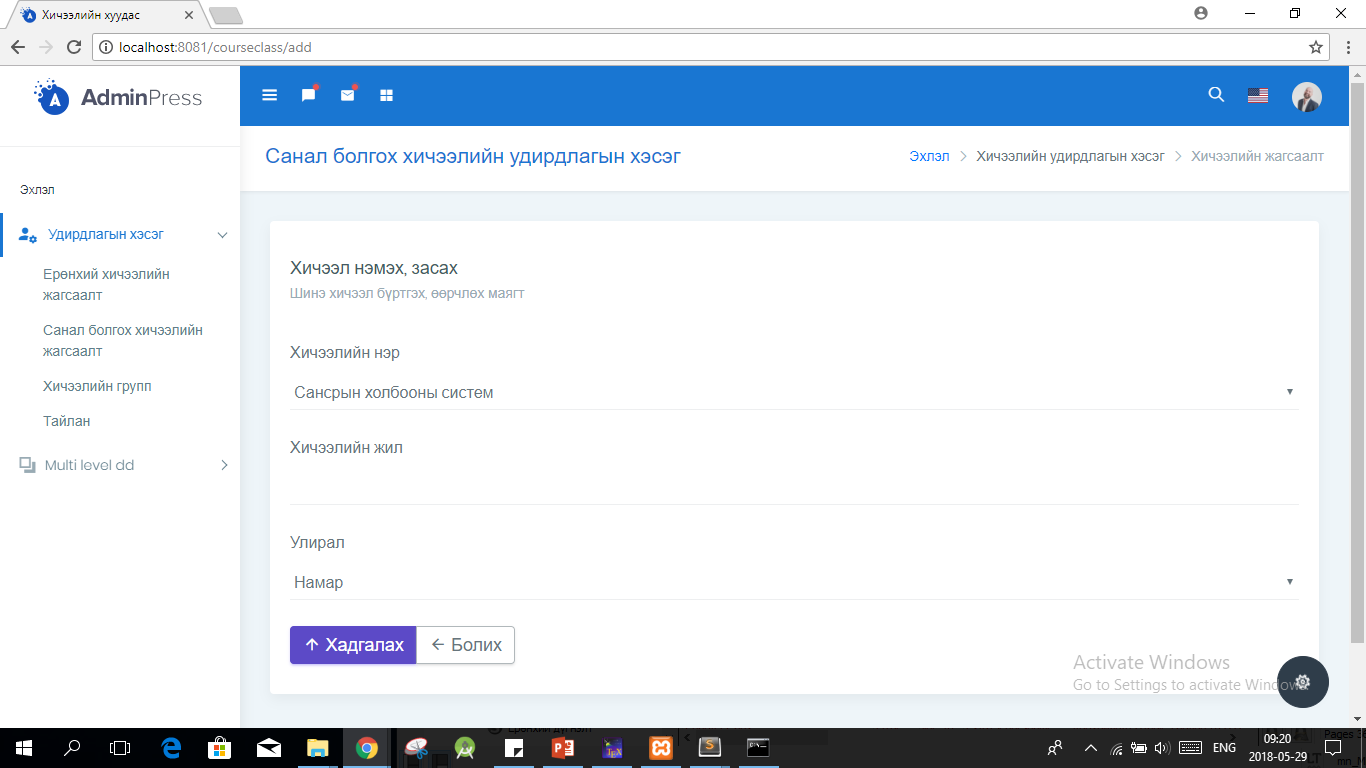
\includegraphics[scale=0.47]{Chart/screen-8}
	\caption[СА-ы ажилтан улирлын хичээл бүртгэх]{СА-ы ажилтан улирлын хичээл бүртгэх}
	\label{text}
\end{figure}
\begin{figure}[!h]
	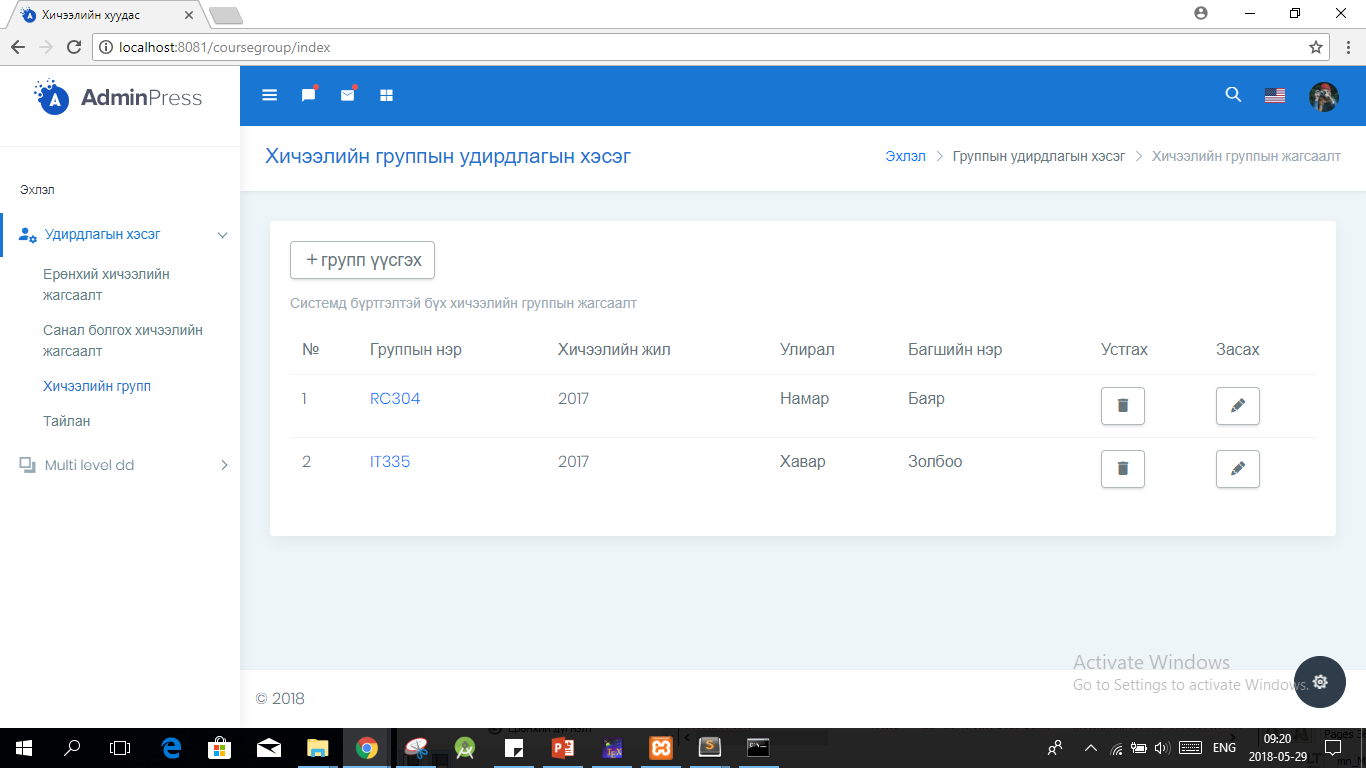
\includegraphics[scale=0.47]{Chart/screen-9}
	\caption[Групп үүсгэх]{Групп үүсгэх}
	\label{text}
\end{figure}
\begin{figure}[!h]
	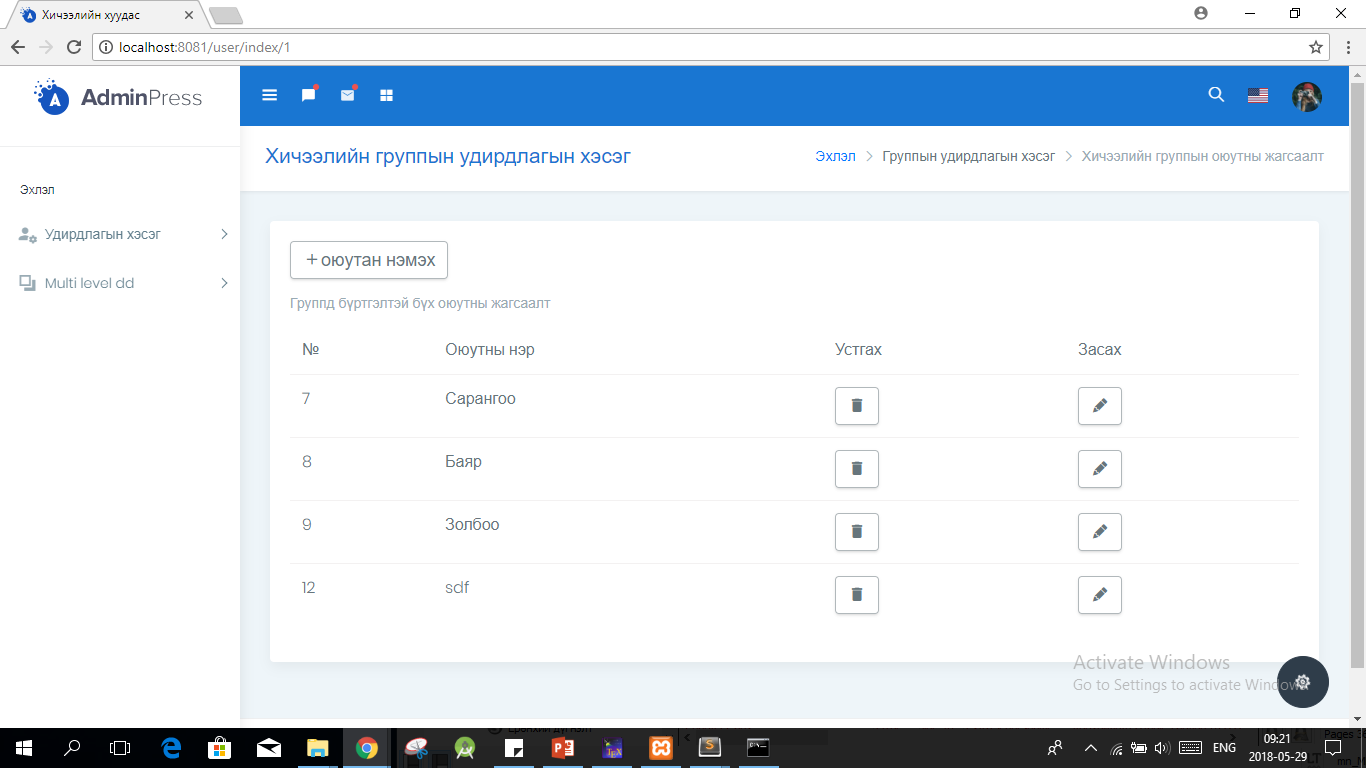
\includegraphics[scale=0.47]{Chart/screen-10}
	\caption[Групп-д гишүүн нэмэх]{Групп-д гишүүн нэмэх}
	\label{text}
\end{figure}
	
%\section{Тайлан, статистик үзүүлэлтийн загвар }
\newpage
\section{Бүлгийн дүгнэлт}
\hspace{1cm}Зохиомжийн хэсэгт өгөгдлийн ерөнхий схем болон өмнөх шинжилгээний класс диаграм дээр үндэслэн зохиомжийн класс диаграм, дарааллын диаграмуудыг гаргасан.
\section{Ерөнхий дүгнэлт}
\hspace{1cm}Мэдээллийн технологи хөгжиж байгаа энэ үед сургуульд хичээлийн веб хуудас үүсгэх нь суралцах зөв арга хэлбэр болж байна.\\
Энэхүү вебийг хийхэд дараах ажлуудыг хийж гүйцэтгэлээ:
\begin{itemize}
	\item Тухайн вебийн талаар судалгаа хийсэн.
	\item CodeIgniter framework –ийн судалгаа хийсэн.
	\item Өгөгдлийн сан болон вебийн дотоод үйл ажиллагааг дүрслэн гаргасан.
	\item Код бичих орчиноо бэлдэх, судалгаа шинжилгээ хийсэн.
\end{itemize}
	
	
